\documentclass{article}
\usepackage{algpseudocode,extramarks,fancyhdr,paralist,amsmath,amsthm,amssymb,mathtools,url,graphicx,pdfpages,tikz,pdfpages,rotating,mathtools, hyperref, bm, hyperref,amsfonts,pgf,mathrsfs,xcolor,comment,mathdots,braket,physics,yhmath,cancel,color,siunitx,array,multirow,amssymb,tabularx,extarrows,booktabs,}
\usetikzlibrary{fadings}
\usetikzlibrary{patterns}
\usetikzlibrary{shadows.blur}
\usetikzlibrary{shapes}
\usepackage[plain]{algorithm}
\usepackage[utf8]{inputenc}

\usetikzlibrary{automata,positioning}

%
% Basic Document Settings
%

\topmargin=-0.45in
\evensidemargin=0in
\oddsidemargin=0in
\textwidth=6.5in
\textheight=9.0in
\headsep=0.25in

\linespread{1.1}

\pagestyle{fancy}
\lhead{\hmwkAuthorName}
\chead{\hmwkClass\ : \hmwkTitle}
\rhead{\firstxmark}
\lfoot{\lastxmark}
\cfoot{\thepage}

\renewcommand\headrulewidth{0.4pt}
\renewcommand\footrulewidth{0.4pt}

\setlength\parindent{0pt}

%
%Proof and theorem structure
%

\theoremstyle{definition} 
\newtheorem{theorem}{Theorem}
\newtheorem{lemma}[theorem]{Lemma}
\newtheorem{claim}[theorem]{Claim}
\newtheorem{corollary}[theorem]{Corollary}
\newtheorem{conjecture}[theorem]{Conjecture}
\newtheorem{definition}[theorem]{Definition}
\newtheorem{example}[theorem]{Example}
\newtheorem{remark}[theorem]{Remark}
\newtheorem{important}[theorem]{Important Note}
\newtheorem{recall}[theorem]{Recall}
\newtheorem{note}[theorem]{Note}
\newtheorem{question}[theorem]{Question}
\newtheorem*{definition*}{Definition}
\newtheorem*{theorem*}{Theorem}
\newtheorem*{claim*}{Claim}

%
%Prefreable integration method
%

\def\upint{\mathchoice%
    {\mkern13mu\overline{\vphantom{\intop}\mkern7mu}\mkern-20mu}%
    {\mkern7mu\overline{\vphantom{\intop}\mkern7mu}\mkern-14mu}%
    {\mkern7mu\overline{\vphantom{\intop}\mkern7mu}\mkern-14mu}%
    {\mkern7mu\overline{\vphantom{\intop}\mkern7mu}\mkern-14mu}%
  \int}
\def\lowint{\mkern3mu\underline{\vphantom{\intop}\mkern7mu}\mkern-10mu\int}

%
% Create Problem Sections
%

\newcommand{\enterProblemHeader}[1]{
    \nobreak\extramarks{}{Problem \arabic{#1} continued on next page\ldots}\nobreak{}
    \nobreak\extramarks{Problem \arabic{#1} (continued)}{Problem \arabic{#1} continued on next page\ldots}\nobreak{}
}

\newcommand{\exitProblemHeader}[1]{
    \nobreak\extramarks{Problem \arabic{#1} (continued)}{Problem \arabic{#1} continued on next page\ldots}\nobreak{}
    \stepcounter{#1}
    \nobreak\extramarks{Problem \arabic{#1}}{}\nobreak{}
}

\setcounter{secnumdepth}{0}
\newcounter{partCounter}
\newcounter{homeworkProblemCounter}
\setcounter{homeworkProblemCounter}{1}
\nobreak\extramarks{Problem \arabic{homeworkProblemCounter}}{}\nobreak{}

%
% Homework Problem Environment
%
% This environment takes an optional argument. When given, it will adjust the
% problem counter. This is useful for when the problems given for your
% assignment aren't sequential. See the last 3 problems of this template for an
% example.
%
\newenvironment{homeworkProblem}[1][-1]{
    \ifnum#1>0
        \setcounter{homeworkProblemCounter}{#1}
    \fi
    \section{Problem \arabic{homeworkProblemCounter}}
    \setcounter{partCounter}{1}
    \enterProblemHeader{homeworkProblemCounter}
}{
    \exitProblemHeader{homeworkProblemCounter}
}

%
% Homework Details
%   - Title
%   - Due date
%   - Class
%   - Section/Time
%   - Instructor
%   - Author
%

\newcommand{\hmwkTitle}{Homework\ \#1}
\newcommand{\hmwkDueDate}{Fri. Sept. 10th}
\newcommand{\hmwkClass}{Classical Mechanics 1}
\newcommand{\hmwkAuthorName}{\textbf{Harlan Heilman}}
\newcommand{\bvec}{\vectorbold}
\newcommand{\di}{\mathrm{d}}
%
% Title Page
%

\title{
    \vspace{2in}
    \textmd{\textbf{\hmwkClass\ }}\\
    \textmd{\textbf{\hmwkTitle\ }}\\
    \normalsize\vspace{0.1in}\small{Due\ on\ \hmwkDueDate\ }\\
    \vspace{3in}
}

\author{\hmwkAuthorName}
\date{}

\renewcommand{\part}[1]{\textbf{\large Part \Alph{partCounter}}\stepcounter{partCounter}\\}

%
% Various Helper Commands
%

% Useful for algorithms
\newcommand{\alg}[1]{\textsc{\bfseries \footnotesize #1}}

% For derivatives
\newcommand{\deriv}[1]{\frac{\mathrm{d}}{\mathrm{d}x} (#1)}

% For partial derivatives
\newcommand{\pderiv}[2]{\frac{\partial}{\partial #1} (#2)}

% Integral dx
\newcommand{\dx}{\mathrm{d}x}

% Alias for the Solution section header
\newcommand{\solution}{\textbf{\large Solution}}

% Probability commands: Expectation, Variance, Covariance, Bias
\newcommand{\E}{\mathrm{E}}
\newcommand{\Var}{\mathrm{Var}}
\newcommand{\Cov}{\mathrm{Cov}}
\newcommand{\Bias}{\mathrm{Bias}}
\newcommand{\lp}{\left(}
\newcommand{\rp}{\right)}

\begin{document}

\maketitle

\pagebreak

\begin{homeworkProblem}
    Consider a rocket of mass $m(t)$ which ejects fuel at a rate of $\dot{m}(t) \leq 0$.  Assume that all of the fuel is ejected with speed $v_e$ directed in the $-x$ direction relative to the rocket

    \begin{enumerate}
        \item Carefully justify the Tsiolkovsky rocket equation derived in class for a rocket moving in one dimension without gravity (or air resistance):
        \[
            v(t) = v(0) + v_e\log\frac{m(0)}{m(t)}.
        \]
        \item This formula is independent of the rate $\dot{m}(t)$ at which fuel is expelled.  Explain how this result is consistent with the simple formula for the velocity of the rocket if all of the fuel were to be immediately eject as one blob with speed $v_e$:
        \[
            v(t>0) = v_i + v_e\frac{m(0) - m(t)}{m(t)}.
        \]
        \item Derive the equation of motion for the rocket moving vertically in a gravitational field.
        \item Solve these equations for a rocket moving vertically in a constant gravitational field.  Assume that $\dot{m}(t) = \dot{m}$ is constant and find the height $z(t)$.
        \item[(e)] Bonus: Briefly estimate how much energy is required to place a payload of $1$kg into a geosynchronous orbit.  How does this depend on the overall mass of the rocket (i.e. is it more efficient to send several small rockets or a single large rocket?\\
    \end{enumerate}
    
    \textbf{Solution}
    Here is a simple drawing of a rocket at some time $t_0$. Here $\di m$ is the infinitesimal mass that is ejected from the rocket after some time $\di t$, $m(t)$ is the mass of the rocket as a function of time, and $v(t)$ the velocity of the rocket as a function of time. We also note that the rocket is loosing mass, thus $\dot{m}(t) \leq 0$.
    \\
    
    \vspace{.5cm}
    \centering
    \tikzset{every picture/.style={line width=0.75pt}} %set default line width to 0.75pt        

    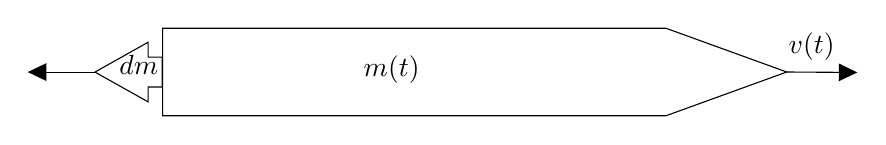
\begin{tikzpicture}[x=0.75pt,y=0.75pt,yscale=-1,xscale=1]
    %uncomment if require: \path (0,300); %set diagram left start at 0, and has height of 300

    %Pentagon Arrow [id:dp3470840385191083] 
    \draw   (149.21,86.82) -- (391.67,86.82) -- (449.9,107.91) -- (391.67,129) -- (149.21,129) -- cycle ;
    %Left Arrow [id:dp967353932333785] 
    \draw   (116.57,107.94) -- (142.19,93.57) -- (142.19,100.76) -- (148.92,100.76) -- (148.92,115.12) -- (142.19,115.12) -- (142.19,122.3) -- cycle ;
    %Straight Lines [id:da38157126997258306] 
    \draw    (449.9,107.91) -- (480.89,108.11) ;
    \draw [shift={(483.89,108.13)}, rotate = 180.36] [fill={rgb, 255:red, 0; green, 0; blue, 0 }  ][line width=0.08]  [draw opacity=0] (8.93,-4.29) -- (0,0) -- (8.93,4.29) -- cycle    ;
    %Straight Lines [id:da780895867331594] 
    \draw    (116.57,107.94) -- (87.22,107.94) ;
    \draw [shift={(84.22,107.94)}, rotate = 360] [fill={rgb, 255:red, 0; green, 0; blue, 0 }  ][line width=0.08]  [draw opacity=0] (8.93,-4.29) -- (0,0) -- (8.93,4.29) -- cycle    ;


    % Text Node
    \draw (244.8,98.8) node [anchor=north west][inner sep=0.75pt]    {$m( t)$};
    % Text Node
    \draw (449.58,87.55) node [anchor=north west][inner sep=0.75pt]    {$v( t)$};
    % Text Node
    \draw (127.13,98.8) node [anchor=north west][inner sep=0.75pt]    {$dm$};
    \end{tikzpicture}

    \raggedright
    \vspace{.5cm}
    \textbf{Part 1} \\
    Suppose we modeled a rocket as a guy sitting in a metal tube throwing infinitesimally small chunks of rock out. Take some snapshot of time before the infinitesimal bit of mass is "thrown out" of the rocket. At this point in time, we see that the momentum of the rocket can be written as 
    \[
        P_i = mv.
    \]
    Now as we step time forward to the point where the small bit of mass gets "thrown out" of the rocket at some speed $v_e$, the momentum can be written as 
    \[
        P_{fR} = (m+\di m)(v+\di v).
    \]
    If we where the guy throwing out the rocks, we would measure the momentum of each rock as 
    \[
        P'_{fM} = v_e\di m
    \]
    but from the laboratory frame, we would measure this momentum as
    \[
        P_{fM} = \di m (v-v_e).
    \]
    Thus by conservation of momentum we find, 
    \[
        m(0)v(0) = (m+\di m)(v+\di v)-\di m (v-v_e)
    \]
    which simplifies to 
    \[
    \begin{split}
        & \frac{\dot{v}\di t}{v_e} = -\frac{\dot{m}\di t}{m}\\
        & \int_0^t\frac{\dot{v}\di t}{v_e} = -\int_0^t\frac{\dot{m}\di t}{m}\\
        & v(t) = v(0) + v_e\log\frac{m(0)}{m(t)}
    \end{split}
    \]
    our desired result. 
    \\
    \textbf{Part 2}\\
    What if the guy throwing out the mass made a mistake and decided to throw the whole fuel canister out at once? If we think about it, we all ready solved this problem, 
    \[
        \frac{\di v}{v_e} = -\frac{\di m}{m}
    \]
    but now we don't have to step time forward anymore as all the mass is ejected all ready. We are being messy with out infinitesimals here, so lets write out explicitly what we mean. Since $\di m$ was the amount of mass that was thrown out of the rocket, it can be written as the difference between the mass of the rocket at some time $t$ and the mass at time $t=0$ (as we want $\di m \leq 0$). In Part 1, we wanted this time to be infinitesimally small, but here we don't care. Similarly, we know that $m$ is nothing but the mass of the rocket. The last differential, $\di v$ is the amount that the rocket speed up by i.e., $v(t) = v_i+\di v$. Thus we can write out equation as 
    \[
        \frac{v(t)-v_i}{v_e} = -\frac{m(t)-m(0))}{m(t)}
    \]
    but this is nothing but our desired result,
    \[
            v(t>0) = v_i + v_e\frac{m(0) - m(t)}{m(t)}.
    \]
    \\
    
    \textbf{Part 3}\\
    Newtons 3rd law gives the equations of motion
    \[
        \dot{p} = -mg
    \]
    but by the fundamental theorem of calculus, we have
    \[ 
        \int_o^t\dot{p}\di t = p(t) - p(0) = -\int_0^tmg\di t.
    \]
    The momentum equations for a rocket free from the effects of gravity still hold, thus we know $p(t)-p(0) = m\di v+v_e\di m$, thus we get a similar differential equation to Part 1
    \[
        \dot{v}\di t =-g\di t -v_e\frac{\dot{m}\di t}{m}.
    \]
    Solving this ode gives,
    \[
        v(t)=v(0)-gt+v_e\log{\frac{m(0)}{m(t)}}
    \]
    \\
    \textbf{Part 4}\\
    Lets define two a new functions the height of the rocket $z(t)$ where $z(0) = z_i$, and $\mu(t)=m(0)/m(t)$. Substituting this into the equation gives,
    \[
        \dot{z}(t) = v_i-gt+v_e\log{\mu(t)}.
    \]
    Note that $\mu(t)\geq 1$. Thus we can write the position function as the integral 
    \[
    \begin{split}
        \int_0^t\dot{z}(t)\di t = z(t) &= z_i + \int_0^t\left(v_i-gt+v_e\sum_{n=1}^\infty(-1)^{n-1}\frac{(\mu(t)-1)^n}{n}\right)\di t.\\
                                &= z_i+ v_it-\frac{1}{2}gt^2+v_e\int_0^t\left(\sum_{n=1}^\infty(-1)^{n-1}\frac{(\mu(t)-1)^n}{n}\right)\di t\\
                                &= z_i+ v_it-\frac{1}{2}gt^2+v_e\sum_{n=1}^\infty(-1)^{n-1}\frac{(\mu(t)-1)^{n+1}}{n(n+1)}.
    \end{split}
    \]
    It is reasonable to assume that this rocket is being launched into space from rest at the surface of the earth, in which case, $z_i = v_i = 0$. Then our result for a rocket being launched from a infinite plane of an earth with no atmosphere can be written as 
    \[
        z(t) \approx -\frac{1}{2}gt^2+\frac{1}{2}v_e\mu(t)^2.
    \]
    \textbf{Part 5}
    
\end{homeworkProblem}

\pagebreak

\begin{homeworkProblem}
    
    As Kepler showed, a particle orbiting in gravitational potential $V(r) = \alpha/r$ will
    move along an ellipse.  Will the center of mass of an extended object also move in a
    perfect ellipse?  Provide a concise and convincing argument that this will be the
    case, or provide a simple counter example.
    \\
    
    \textbf{Solution}\\
    
    Suppose we had an object that could be described by a line of mass, analogous to a finite length wire of charge. From E\&M, we see that the electric field of a finite wire can be described as,
    \[
        E = \frac{\lambda}{2\pi\epsilon_0r}
    \]
    but this is analogous to a Gravitational field described by
    \[
        \bvec F = \frac{Gm\lambda}{2r}\hat{\bvec r} = \frac{Gm}{2lr}\hat{\bvec r}
    \]
    where $l$ is the length of the wire. If we put this object into the  But now the potential is no longer $\alpha/r$ dependant, but instead is $\alpha\log{r}$ dependant. We define the distance from the origin to the "sun" as $r_1$, and the distance from the origin to the center of the wire of mass $r_2$. By newtons laws, we get the equations of motion described by,
    \[
        m_1\ddot{\bvec r}_1 = \frac{\alpha}{r_{12}}\frac{\bvec r_1-\bvec r_2}{r12}
    \]
    \[
        m_2\ddot{\bvec r}_2 = \frac{\beta}{r_{12}^2}\frac{\bvec r_2-\bvec r_1}{r12}
    \]
    We don't see this in the case of spherical masses, just how in E\&M we find the Electric Field outside of a solid insulating sphere as 
    \[
        E = \frac{kQ}{r^2}.
    \]
    From far away, these things are approximately point charges/masses compared to the sizes of orbits. 
\end{homeworkProblem}

\pagebreak

\begin{homeworkProblem}
    Throughout the course we will visit the problem of a Harmonic Oscillator: i.e. the motion of a particle of mass $m$ in a potential $V(r) = \tfrac{1}{2}kr^2$ which might represent a ball connected to an anchored spring with spring constant $k$.  We shall revisit this problem in all formalisms and use it as a basis for understanding chaotic dynamics.
    
    \begin{itemize}
        \item [(a)] Use the effective potential to show that all orbits are bound and that $E$ must exceed $E_{\text{min}} = \sqrt{kl^2/m}$ where $l$ is the angular momentum of the system.
        \item [(b)] Verify that the orbit is a closed ellipse with the origin at the center of the potential.  (Compare your result with the formulas in the book for problem 1.10 (b).)
        \item [(c)] Prove that the period is independent of the energy and angular momentum.  Could you have anticipated this from simple arguments? Discuss the significance of this result.
    \end{itemize}
    
    \textbf{Solution}
    
    Let us start out with looking at the equations of motion that arise from Newtons laws. Defining the origin as the center of the potential, a frame that does not move, let $r$ be the position vector from the center of the potential well to the ball. Then we can describe the motion via Newtons Laws as
    \[
        m\ddot{\bvec r} = -\grad V(r) = -kmr\frac{\bvec r}{|r|}.
    \]
    \\
    \textbf{Part(a)} \\
    Lets start out with the definition of angular momentum
    \[
        \bvec L = \bvec r\cp\bvec p,
    \]
    In consequence, the force and the vector $\bvec r$ are parallel, and thus the torque vanishes. This means the the angular momentum is fixed, and we have the following identities,
    \[
        \bvec r\vdot\bvec l = \bvec r\vdot(\bvec r\cp\bvec p) = 0
    \]
    \[
        \bvec p\vdot\bvec l = \bvec r\vdot(\bvec r\cp\bvec p) = 0.
    \]
    Thus, the momentum of the object is strictly planar.
    
    We now turn to conservation of Energy, 
    \[
        E = \frac{1}{2}m(\dot{x}^2+\dot{y}^2)+V(r)
    \]
    where the planar motion can be described by $r,\phi$, with
    \[
        x = r\cos{\phi}, y = r\sin{\phi}.
    \]
    Thus the energy can be written as 
    \[
        E = \frac{1}{2}m(\dot{r}^2+r^2\phi^2 +V(r) = \frac{1}{2}m\lp\dot{r}^2+\frac{l^2}{m^2r^2}\rp+V(r) = \frac{1}{2}m\dot{r}^2+V_e
    \]
    where 
    \[
        V_e = \frac{l^2}{2m^2r^2}+\frac{kr^2}{2}.
    \]
    We set the kinetic energy equal to zero and minimize the effective potential. This gives us the point of lowest energy $r_0 = \frac{l}{m\sqrt{k}}$, and plugging this in gives
    \[
        E_{min} = \sqrt{kl^2/m}.
    \]
    \\
    
    \textbf{Part (b)} \\
    From Fetter and Walecka, we know that for $u = 1/r$,
    \[
        \phi-\phi_0 = \mp \int^u\di u\left[\frac{2mE}{l^2}-u^2-\frac{km}{l^2u^2}\right]^{-1/2}u
    \]
    but we substitute $v = u^2$ s.t $\di v = 2u\di u$ giving us
    \[
        \phi-\phi_0 = \mp \frac{1}{2}\int\di v\left[\frac{2mE}{l^2} - \frac{km}{l^2}v-v^2\right]^{-1/2}.
    \]
    But we let $c = -km/l^2, b = 2mE/l^2$, and perform the substitution resulting in the form 
    \[
        \phi-\phi_0 = \mp \frac{1}{2}\int\di v\left[v^2-\lp c+\frac{b^2}{4}\rp\right]^{-1/2}
    \]
    and lastly, let $\zeta = v(\sqrt{c+b^2/4})^{-1}$ resulting in the integral 
    \[
        2\Delta\phi = \mp \frac{1}{2}\int\di \zeta\left[1-\zeta\right]^{-1/2} = \pm\cos^{-1}(\zeta).
    \]
    Working backwards, we get the solution
    \[
    \begin{split}
        2\Delta\phi &= \pm\cos^{-1}\lp\frac{\frac{1}{r^2}-\frac{mE}{l^2}}{\left[\frac{m^2E^2}{l^4}-\frac{km}{l^2}\right]^{1/2}}\rp\\
        \frac{1}{r^2}-\frac{mE}{l^2} &= \pm \left[\frac{m^2E^2}{l^4}-\frac{km}{l^2}\right]^{1/2}\cos{(2\Delta\phi)}\\
        \frac{1}{r^2} &= \lp\frac{km}{l^2}\rp^ {1/2}\left[\frac{E}{E_{min}}-\lp\frac{E^2}{E_{min}^2}-1\rp^{1/2}\right] \cos{2\Delta\phi}
    \end{split}
    \]
    This gives us the equation of a conic section in polar coordinates. However, to show that these are all ellipses we should show that $0<\varepsilon<1$ for eccentricity $\varepsilon$. From the equations in Fetter and Walecka we have $E/E_{min} = \cosh{\zeta}$ and we will take this as a fact. Let $\alpha = \lp\frac{km}{l^2}\rp^ {1/2}$, the equation becomes
    \[
    \begin{split}
        \frac{1}{r^2} &= \alpha\left[\cosh{\zeta}-(\cosh{\zeta}-1)^{1/2} \right]\cos{2\phi}\\
                      &= \alpha\left[\cosh{\zeta}-(\cosh{\zeta}-1)^{1/2} \right](\cos^2{\phi}-1)\\
                      &=\alpha\left[(\cosh{\zeta}+\sinh{\zeta})+(2\cosh{\zeta}+2\sinh{\zeta}\right)\cos{\phi}]\\
                      &=\alpha e^{\zeta}[1-(1-e^{-2\zeta})\cos^2{\phi}]
    \end{split}
    \]
    where $\varepsilon^2 = 1-e^{-2\zeta}$. We see that the eccentricity is only $0$ if the $\zeta = 0$, or the systems energy is the minimal energy. In order for the eccentricity to be one, $\zeta$ must approach infinity, and we see the energy of the object in motion also approaches infinity. 
\end{homeworkProblem}

\pagebreak

\begin{homeworkProblem}
    A uniform beam of particles with energy $E$ is scattered by an attractive (top-hat or
    spherical square-well) central potential:
    \[
    V(r) = \begin{cases}
                -V_0 & r < a\\
                0 & r > a
            \end{cases}
    \]
    Show that the orbit of a particle is identical to a light ray refracted by a sphere of
    radius $a$ with a particular index of refraction $n$ (see the book). Compute the
    differential cross-section and show that it is
    \[
    \frac{\mathrm{d}\sigma}{\mathrm{d}\Omega} = \frac{n^2 a^2}{4\cos(\tfrac{1}{2}\theta)}
    \frac{\left[n\cos(\tfrac{1}{2}\theta) - 1\right]\left(n-\cos\tfrac{1}{2}\theta\right)}{\left(1+n^2 - 2n + \cos\tfrac{1}{2}\theta\right)^2}
    \]
    Compute the total cross-section $\sigma$.
    \\
    
    \textbf{Solution}\\
    

\tikzset{every picture/.style={line width=0.75pt}} %set default line width to 0.75pt        

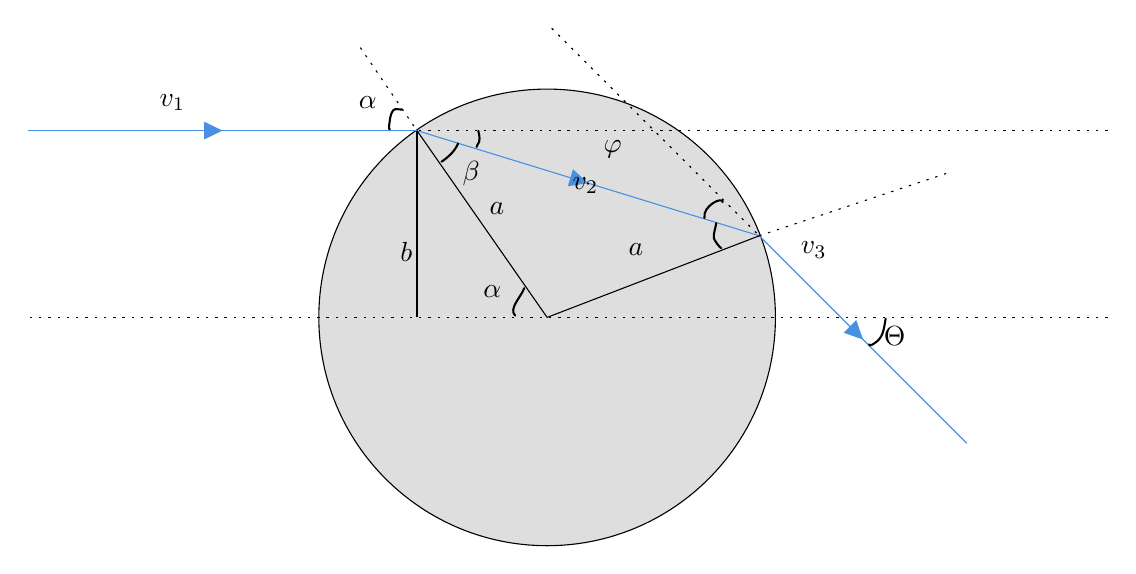
\begin{tikzpicture}[x=0.75pt,y=0.75pt,yscale=-1,xscale=1]
%uncomment if require: \path (0,300); %set diagram left start at 0, and has height of 300

%Shape: Circle [id:dp21660419029682076] 
\draw  [fill={rgb, 255:red, 0; green, 0; blue, 0 }  ,fill opacity=0.13 ] (220,140) .. controls (220,79.25) and (269.25,30) .. (330,30) .. controls (390.75,30) and (440,79.25) .. (440,140) .. controls (440,200.75) and (390.75,250) .. (330,250) .. controls (269.25,250) and (220,200.75) .. (220,140) -- cycle ;
%Straight Lines [id:da13215554471957547] 
\draw [color={rgb, 255:red, 74; green, 144; blue, 226 }  ,draw opacity=1 ]   (80,50) -- (267.29,50) ;
\draw [shift={(173.65,50)}, rotate = 180] [fill={rgb, 255:red, 74; green, 144; blue, 226 }  ,fill opacity=1 ][line width=0.08]  [draw opacity=0] (8.93,-4.29) -- (0,0) -- (8.93,4.29) -- cycle    ;
%Straight Lines [id:da8679191792982661] 
\draw [color={rgb, 255:red, 74; green, 144; blue, 226 }  ,draw opacity=1 ]   (267.29,50) -- (432.23,100.68) ;
\draw [shift={(349.76,75.34)}, rotate = 197.07999999999998] [fill={rgb, 255:red, 74; green, 144; blue, 226 }  ,fill opacity=1 ][line width=0.08]  [draw opacity=0] (8.93,-4.29) -- (0,0) -- (8.93,4.29) -- cycle    ;
%Straight Lines [id:da09297503477012903] 
\draw    (267.29,50) -- (330,140) ;
%Straight Lines [id:da5872871299399809] 
\draw  [dash pattern={on 0.84pt off 2.51pt}]  (600,140) -- (80,140) ;
%Straight Lines [id:da524308912071813] 
\draw  [dash pattern={on 0.84pt off 2.51pt}]  (600,50) -- (267.29,50) ;
%Straight Lines [id:da582874385457476] 
\draw    (267.29,140) -- (267.29,50) ;
%Straight Lines [id:da06417991954184865] 
\draw [color={rgb, 255:red, 74; green, 144; blue, 226 }  ,draw opacity=1 ]   (432.23,100.68) -- (532.23,200.68) ;
\draw [shift={(482.23,150.68)}, rotate = 225] [fill={rgb, 255:red, 74; green, 144; blue, 226 }  ,fill opacity=1 ][line width=0.08]  [draw opacity=0] (8.93,-4.29) -- (0,0) -- (8.93,4.29) -- cycle    ;
%Straight Lines [id:da15162907945876913] 
\draw    (330,140) -- (432.23,100.68) ;
%Straight Lines [id:da8136998536394779] 
\draw  [dash pattern={on 0.84pt off 2.51pt}]  (332.23,0.68) -- (432.23,100.68) ;
%Shape: Free Drawing [id:dp17789759297448993] 
\draw  [color={rgb, 255:red, 0; green, 0; blue, 0 }  ][line width=0.75] [line join = round][line cap = round] (287.11,56.2) .. controls (285.59,59.86) and (282.41,62.8) .. (279.11,65) ;
%Shape: Free Drawing [id:dp5090035130280766] 
\draw  [color={rgb, 255:red, 0; green, 0; blue, 0 }  ][line width=0.75] [line join = round][line cap = round] (411.51,94.6) .. controls (411.11,97) and (410.13,99.37) .. (410.31,101.8) .. controls (410.37,102.58) and (413.54,106.98) .. (413.91,106.6) ;
%Shape: Free Drawing [id:dp12918191732067097] 
\draw  [color={rgb, 255:red, 0; green, 0; blue, 0 }  ][line width=0.75] [line join = round][line cap = round] (493.11,140.6) .. controls (492.34,144.46) and (492.18,148.77) .. (489.11,151.4) .. controls (488.02,152.33) and (485.11,154.44) .. (485.11,153) ;
%Shape: Free Drawing [id:dp8843507582489494] 
\draw  [color={rgb, 255:red, 0; green, 0; blue, 0 }  ][line width=0.75] [line join = round][line cap = round] (296.83,50.09) .. controls (297.38,52.29) and (298.03,55.28) .. (296.43,56.89) .. controls (295.99,57.33) and (296.03,58.79) .. (296.03,57.69) ;
%Shape: Free Drawing [id:dp06270004417971453] 
\draw  [color={rgb, 255:red, 0; green, 0; blue, 0 }  ][line width=0.75] [line join = round][line cap = round] (405.8,92.09) .. controls (404.83,86.26) and (414.6,81.49) .. (414.6,84.49) ;
%Straight Lines [id:da04851222168415448] 
\draw  [dash pattern={on 0.84pt off 2.51pt}]  (240,10) -- (267.29,50) ;
%Shape: Free Drawing [id:dp015300041651448604] 
\draw  [color={rgb, 255:red, 0; green, 0; blue, 0 }  ][line width=0.75] [line join = round][line cap = round] (319,125.91) .. controls (317.37,130.26) and (311.32,135.83) .. (314.6,139.11) ;
%Shape: Free Drawing [id:dp2493424132408173] 
\draw  [color={rgb, 255:red, 0; green, 0; blue, 0 }  ][line width=0.75] [line join = round][line cap = round] (260.2,39.86) .. controls (258.73,39.99) and (256.69,39.09) .. (255.8,40.26) .. controls (254.13,42.44) and (254.25,45.55) .. (253.8,48.26) .. controls (253.73,48.67) and (254.2,49.88) .. (254.2,49.46) ;
%Straight Lines [id:da3166391160227007] 
\draw  [dash pattern={on 0.84pt off 2.51pt}]  (432.23,100.68) -- (522.23,70.68) ;

% Text Node
\draw (491,143.4) node [anchor=north west][inner sep=0.75pt]    {$\Theta $};
% Text Node
\draw (238,32.4) node [anchor=north west][inner sep=0.75pt]    {$\alpha $};
% Text Node
\draw (298,123.4) node [anchor=north west][inner sep=0.75pt]    {$\alpha $};
% Text Node
\draw (301,83.4) node [anchor=north west][inner sep=0.75pt]    {$a$};
% Text Node
\draw (258,102.4) node [anchor=north west][inner sep=0.75pt]    {$b$};
% Text Node
\draw (368,103.4) node [anchor=north west][inner sep=0.75pt]    {$a$};
% Text Node
\draw (356,53.4) node [anchor=north west][inner sep=0.75pt]    {$\varphi $};
% Text Node
\draw (288,63.4) node [anchor=north west][inner sep=0.75pt]    {$\beta $};
% Text Node
\draw (142,31.4) node [anchor=north west][inner sep=0.75pt]    {$v_{1}$};
% Text Node
\draw (341,71.4) node [anchor=north west][inner sep=0.75pt]    {$v_{2}$};
% Text Node
\draw (451,102.4) node [anchor=north west][inner sep=0.75pt]    {$v_{3}$};


\end{tikzpicture}

    First let us note that once a particle passes though the potential field and out the other side, by conservation of momentum
    \[
        \bvec p_i = p_{xi} = p_{xf}+p_{yf} = \bvec p_f.
    \]
    Now at the boundary as the particle enters the potential, and immediately has some change in momentum due to the instantaneously present force. We define the new momentum once the particle enters the potential $\bvec P'=m\bvec v_1$ where as before the momentum was $\bvec P = m\bvec v_0$. However, we define the momentum of these rays as uniform and traveling only in the $\hat{i}$ direction. Thus we see that by angular momentum conservation across the boundary, 
    \[\begin{split}
        \bvec a\cp m\bvec v_0 &= \bvec a\cp m\bvec v_1\\
        [mv_0a\sin{\alpha}]\hat{k}&= \hat{k}[amv_1\sin{(\alpha-\phi)}]
    \end{split}\]
    where we define the potential centered at $r=0$, $\alpha$ is the angle between the surface normal and the incident particle, and $\phi$ is the new angle that the particle travels at once it enters the potential. We define $\beta = \alpha - \phi$ and thus we have the equation of Snell's law
    \[
        \sin{\alpha} = n\sin{\beta}
    \]
    with $n = v_1/v_2$. But by conservation of energy, the energy of the particle before it enters the potential is described by
    \[
        E = \frac{mv_0^2}{2m}
    \]
    and the velocity in the medium is 
    \[
        E = \frac{mv_1^2}{2m}-V_0
    \]
    and thus we have the relation
    \[
        n^2 = 1+V_0/E = \frac{E+V_0}{E}.
    \]
    Lastly, since we know that $v_1 = v_3$, we can use the geometry to get the impact parameter $\Theta$ can be given as 
    \[
        \Theta = 2(\alpha-\beta).
    \]
    This function can be written as a function of $b$ since from the geometry, we see that $\sin{\alpha} = b/a$ resulting in 
    \[
        \frac{b}{a} = \sin(\Theta/2+\beta).
    \]
    But after some algebra, we see that the equation can be massaged into terms purely based purely on the geometry of the problem
    \[
        b = \frac{an\sin{\Theta/2}}{\sqrt{1+n^2-2n\cos{\Theta/2}}}
    \]
    Thus plugging it into an equation for differential cross section, we get 
    \[
    \begin{split}
        \frac{\di \sigma}{\di \Omega} &= \frac{a^2n^2\sin{\Theta/2}}{2\sin(\Theta)}\frac{\left[n\cos(\tfrac{1}{2}\Theta) - 1\right]\left[n-\cos\tfrac{1}{2}\Theta\right]}{(1+n^2+2n\cos{\Theta/2})^{2}}\\
                                      &=\frac{n^2 a^2}{4\cos(\tfrac{1}{2}\Theta)}
        \frac{\left[n\cos(\tfrac{1}{2}\Theta) - 1\right]\left(n-\cos\tfrac{1}{2}\Theta\right)}{\left(1+n^2 - 2n + \cos\tfrac{1}{2}\Theta\right)^2}
    \end{split}
    \]
    as expected. We now calculate the total cross section area as 
    \[
        \sigma = \int_{0}^{\pi}2\pi b\frac{\di b}{\di \theta}\di \theta = 2\pi \left[\lp\frac{an\sin{\Theta/2}}{\sqrt{1+n^2-2n\cos{\Theta/2}}}\rp^2\right]_o^\pi = 2\pi a^2\frac{n^2}{1+n^2}.
    \]
    But by definition, 
    \[
        \frac{n^2}{1+n^2} = \frac{E+V_0}{2E+V_0} \rightarrow 1/2
    \]
     as $E\rightarrow V_0$, and thus we have the result $\sigma = \pi a^2$.
\end{homeworkProblem}



\end{document}
